\chapter{Cylindrical Simulations to Study the Effect of Beam Radius in Direct-Drive}



%###############################################################################################################################
%###############################################################################################################################
%###############################################################################################################################
\section{Introduction to Beam Radius in Direct-Drive Inertial Confinement Fusion}%
\label{sec:Res1_Beamrad_intro}

\begin{figure}[t!]
    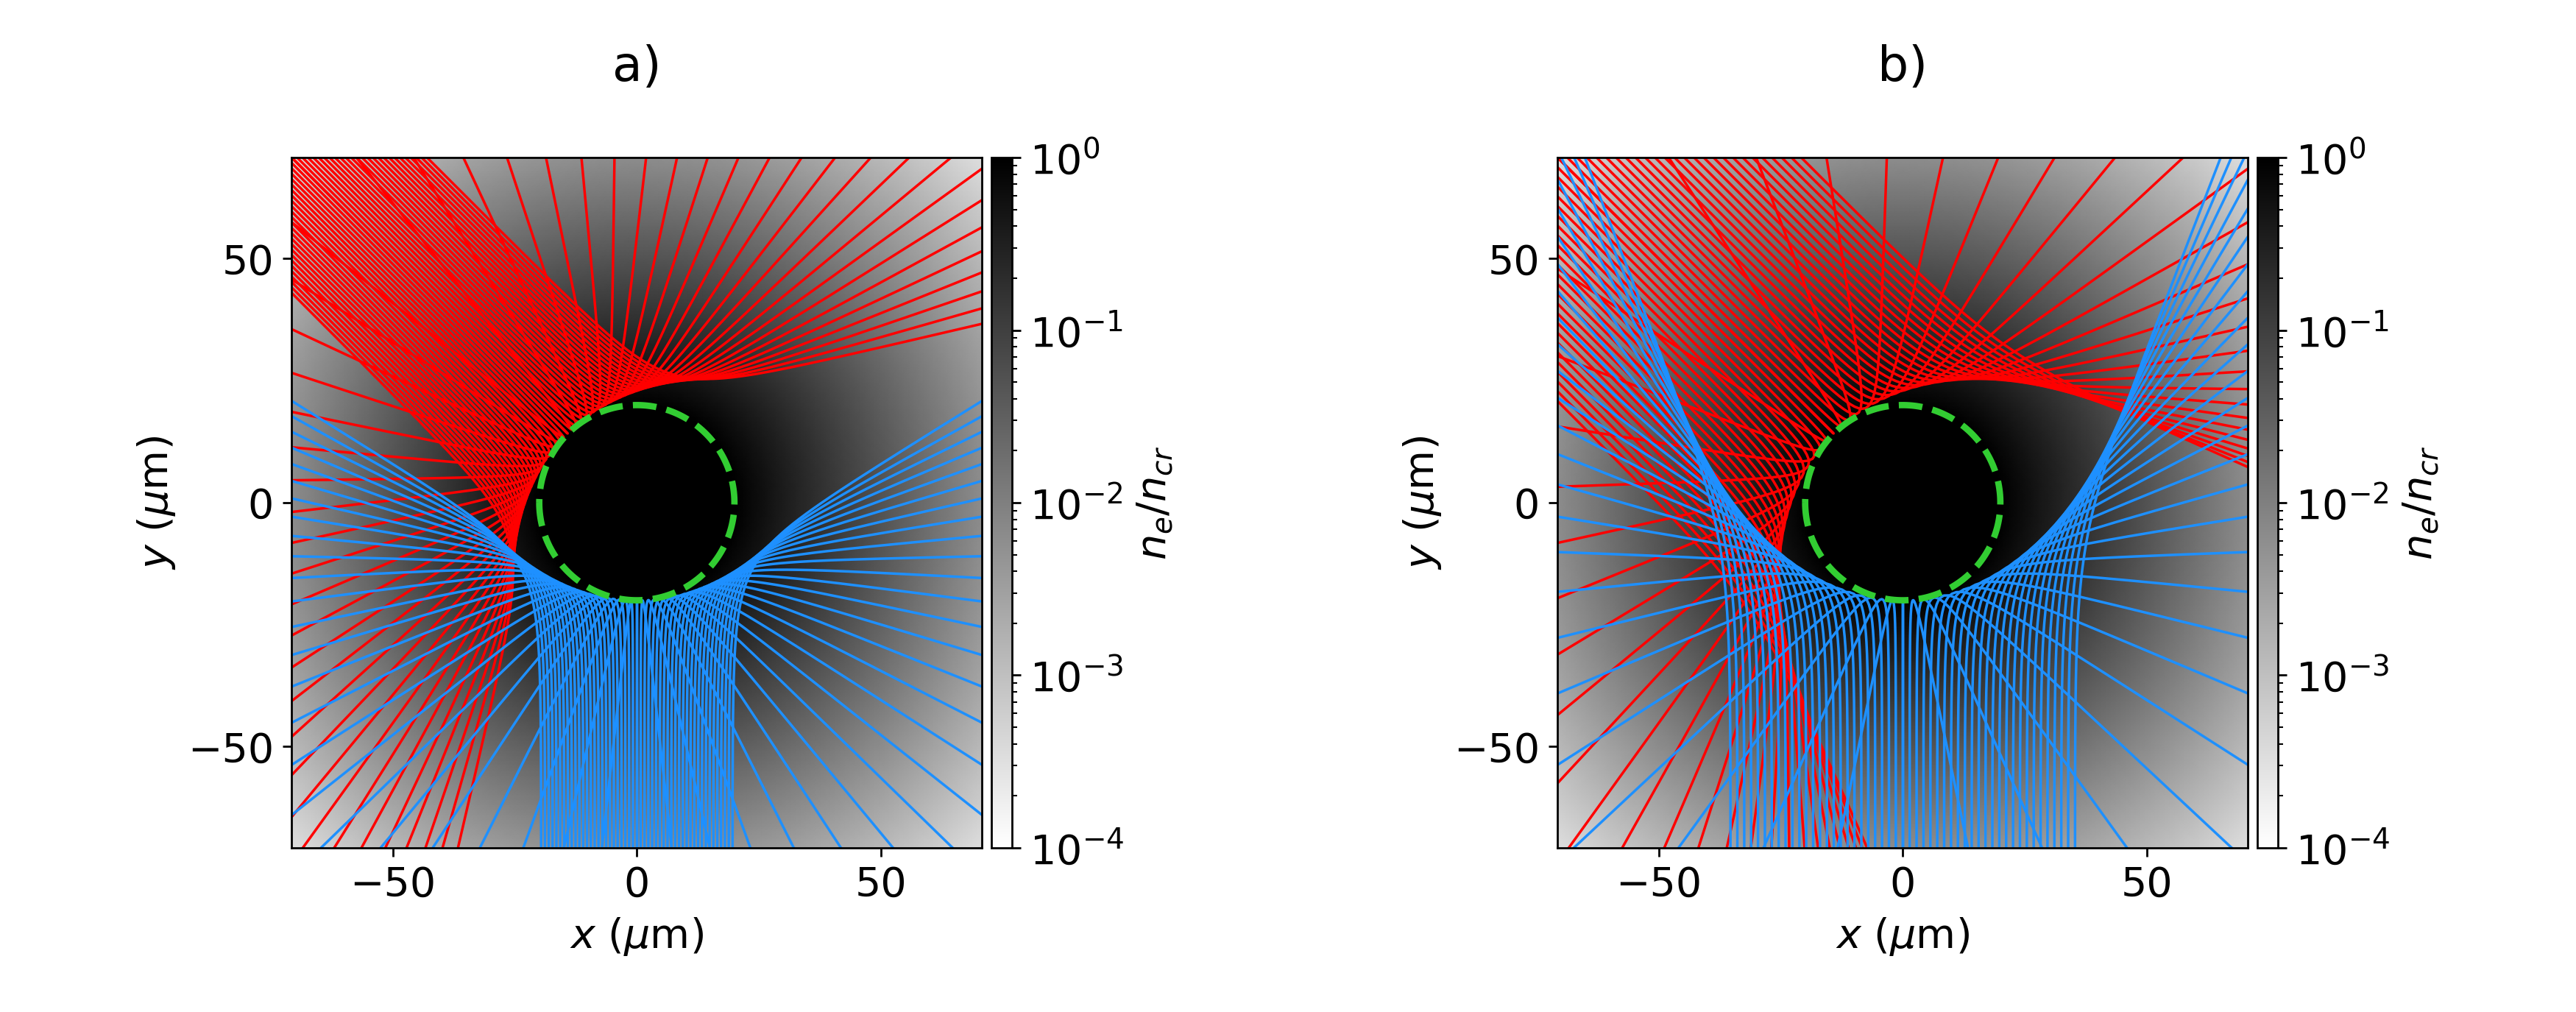
\includegraphics[width=\linewidth]{Results1/Images/RbRt_beam_overlap.png}
    \centering
    \caption{The trajectory of rays from two beams with Beam radii.
    The density profile for both simulations is $n_e=n_{\text{cr}}\exp{[ -(r_{\mu\text{m}}-20)/100 ]}$.
    Panels a) and b) plot rays from beams with widths $\sigma=10$ and $18\ \mu\text{m}$ respectively.}%
    \label{fig:Res1_RbRt_beam_overlap}
\end{figure}




%################################################################################
%################################################################################
\subsection{Statistical Modelling of \textsc{Omega} Direct-Drive Implosions}%
\label{sec:Res1_OMEGA_stat_modelling}


%################################################################################
%################################################################################
\subsection{Beam Radius in Statistical Modelling}%
\label{sec:Res1_OMEGA_stat_modelling_RbRt}


%###############################################################################################################################
%###############################################################################################################################
%###############################################################################################################################
\section{Cylindrical Simulation Platform for Beam Radius Parameter Scan}%
\label{sec:Res1_CylRbRt_platform}


%################################################################################
%################################################################################
\subsection{Assumptions and Validity of the Cylindrical Simulation Platform}%
\label{sec:Res1_platformvalidity}


%################################################################################
%################################################################################
\subsection{Problems with Traditional Methods of Investigating Beam Radius Parameter Computationally}%
\label{sec:Res1_computational_difficulties}


%################################################################################
%################################################################################
\subsection{Pulse Shape and Target Initial Conditions}%
\label{sec:Res1_initialconditions}


%################################################################################
%################################################################################
\subsection{1-D Implosion Tuning}%
\label{sec:Res1_1D_tuning}


%###############################################################################################################################
%###############################################################################################################################
%###############################################################################################################################
\section{CBET Induced Modal Flips in Power Deposition Asymmetries}%
\label{sec:Res1_PdepR_CBET_asymm}


%################################################################################
%################################################################################
\subsection{Deposition Asymmetries in the Absence of CBET}%
\label{sec:Res1_noCBET_asymmetries}


%################################################################################
%################################################################################
\subsection{CBET Imprint on Incident Field}%
\label{sec:Res1_CBET_imprint}


%################################################################################
%################################################################################
\subsection{Modal Flips of Power Deposition Asymmetries}%
\label{sec:Res1_ModalFlip}


%###############################################################################################################################
%###############################################################################################################################
%###############################################################################################################################
\section{Stagnation State Asymmetry}%
\label{sec:Res1_StagnationAsymm}


%################################################################################
%################################################################################
\subsection{Stagnation State Asymmetry Trend with Beam Radius}%
\label{sec:Res1_stagnation_asymm_trend}


%################################################################################
%################################################################################
\subsection{Hotspot Profiles}%
\label{sec:Res1_HS_profiles}


%################################################################################
%################################################################################
\subsection{Time Resolved Asymmetry Growth}%
\label{sec:Res1_time_res_growth}


%###############################################################################################################################
%###############################################################################################################################
%###############################################################################################################################
\section{Conclusions}%
\label{sec:Res1_Conclusions}


%################################################################################
%################################################################################
\subsection{Summary of work}%
\label{sec:Res1_Summary}


%################################################################################
%################################################################################
\subsection{Future Work}%
\label{sec:Res1_future}